%%
%% Now we have to get the source code in as a set of Appendices.
%% Source code will be Appendix A, with each file numbered X.y
%%
%\appendix

%%
%% -> \Chapter will cause the next bit to be labelled Appendix A
%% -> \section will give us A.1, \subsection A.1.1 etc.
%%
%% I suggest a section for each program and a subsection for each file
%% in the program.  Alternatively, a Chapter for each program, a
%% section for each library and a subsection for each file.
%%

\chapter{Sample Quality}
\label{appendix:sample_checking}

\section{Sample Correlation}
\label{appendix:sample_correlation}

Samples were excluded from expression analysis based on sample correlations and the clustering analysis presented below, as described in Section~\ref{methods:sample_qc}.  

\begin{figure*}[!ht]
%\begin{mdframed}
  \begin{center}
  \resizebox{0.75 \textwidth}{!}{
    \includegraphics{Raw(log)_Corr_eudist_Cut_part_Pub.png}
   }
   \end{center}
   \caption[Correlation profiles of removed samples]{\small \textbf{Correlation profiles of removed samples.} Correlation matrix heatmap (Euclidean distance) of all samples in TCGA breast cancer dataset (left) clustered for all samples against removed samples (top): tissue source site (TSS), sample type with reds for tumour and greens for normal, patient (A2QH in pink), with varied analyte and plate (corresponding to batch in Table~\ref{tab:qc}). Excluded samples cluster at the bottom and annotation (left) show  shared properties between samples in the dataset.
   }
\label{fig:corr_map_part}
%\end{mdframed}
\end{figure*}

\begin{figure*}[!ht]
%\begin{mdframed}
  \begin{center}
  \resizebox{\textwidth}{!}{
    \includegraphics{Raw(log)_Corr_eudist_Ann_Pub.png}
   }
   \end{center}
   \caption[Correlation analysis and sample removal]{\small \textbf{Correlation analysis and sample removal.} Correlation matrix heatmap (Euclidean distance) of all samples in TCGA breast cancer dataset against each other annotated for sample clinical data: sample type, tissue type, tumour stage, Estrogen receptor (IHC) and intrinsic subtype (from the PAM50 method). CDH1 somatic mutation, gene expression, and status for SLIPT prediction are also annotated. Discrete variables are coloured as displayed in the legend and continuous variables on a blue-red scale as shown in the colour key. Trimmed samples cluster at the bottom of the heatmap and the colour bars of the left show which were removed for quality concerns.}
\label{fig:corr_map}
%\end{mdframed}
\end{figure*}

\clearpage

\section{Replicate Samples in TCGA Breast}
\label{appendix:replicate_samples}

Replicate samples were picked where possible from the TCGA breast cancer gene expression data to examine for sample quality. Independent samples of the same tumour are expected to have very high Pearson's correlation between their expression profiles unless there were issues with sample collection or preparation and are thus an indicator of sample quality. The log-transformed raw read counts for replicate samples were examined in Figures~\ref{fig:rep_cutcut}\nobreakdash--\ref{fig:rep_keepcut}. These were examined before normalisation which would be expected to increase sample concordance.

Another consideration are the samples which were removed for quality concerns (in Section~\ref{methods:sample_qc}). While these were selected by unbiased hierarchical clustering (See Figure~\ref{fig:corr_map}), it is notable that many of the exluded (tumour) samples were performed in replicate despite relatively few replicate samples in the overall dataset. These samples correlate poorly with the rest of the dataset, in addition to with replicate samples.

\begin{figure*}[!hb]
%\begin{mdframed}
  \centering
  \resizebox{0.3\textwidth}{!}{
    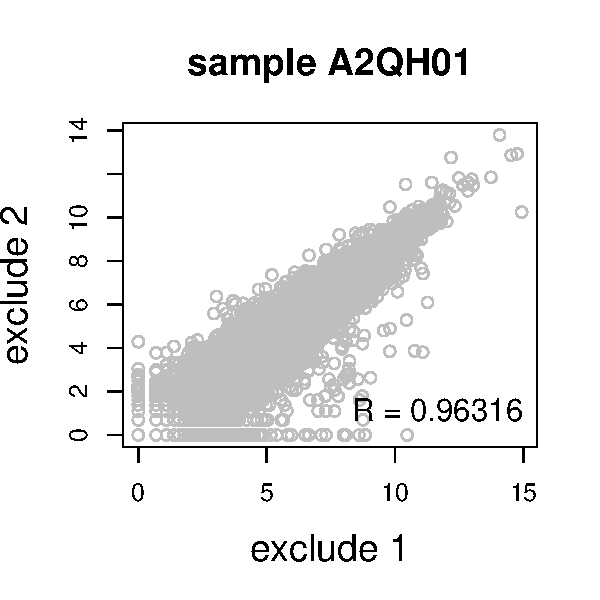
\includegraphics{Rep_picking_CutCut2.pdf}
   }
    \caption[Replicate excluded samples]{\small \textbf{Replicate excluded samples.} Both tumour samples of patient A2QH were excluded as they were poorly correlated with other samples, although they are highly similar to each other as shown by Pearson's correlation of log-raw counts.
}
\label{fig:rep_cutcut}
%\end{mdframed}
\end{figure*}

\begin{figure*}[!ht]
%\begin{mdframed}
           \begin{center}
%
        \subcaptionbox{Remaining triplet}{%
           \label{fig:rep_keepcut:A26J:first}
           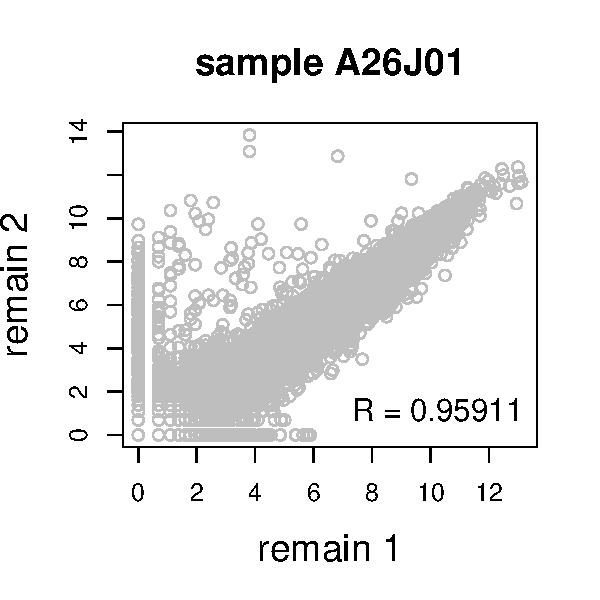
\includegraphics[width=0.3\textwidth]{Rep_picking_KeepKeep(1).pdf}
        }%
        \subcaptionbox{Remaining triplet}{%
           \label{fig:rep_keepcut:A26J:second}
           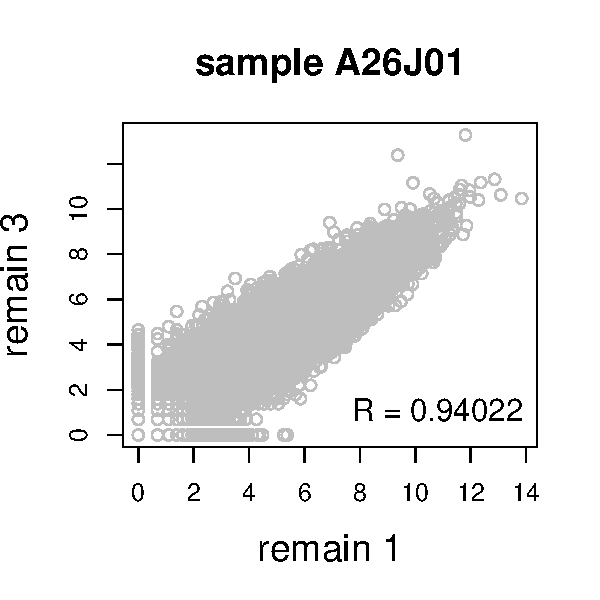
\includegraphics[width=0.3\textwidth]{Rep_picking_KeepKeep(2).pdf}
        }%
        \subcaptionbox{Remaining triplet}{%
           \label{fig:rep_keepcut:A26J:third}
           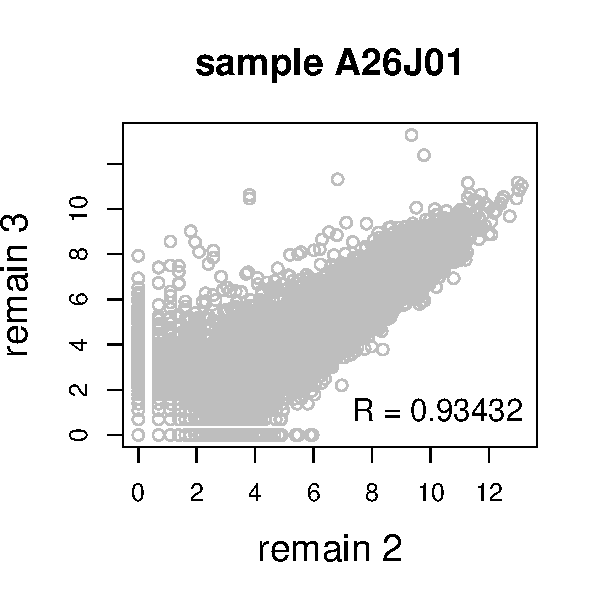
\includegraphics[width=0.3\textwidth]{Rep_picking_KeepKeep(3).pdf}
        }%
%

%
        \subcaptionbox{Remaining pair}{%
           \label{fig:rep_keepcut:A13G}
           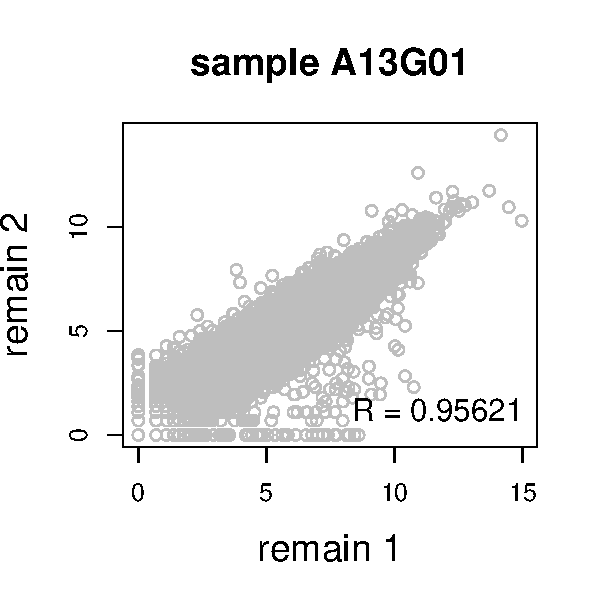
\includegraphics[width=0.3\textwidth]{Rep_picking_KeepKeep(4).pdf}
        }%
        \subcaptionbox{Remaining pair}{%
           \label{fig:rep_keepcut:A26F}
           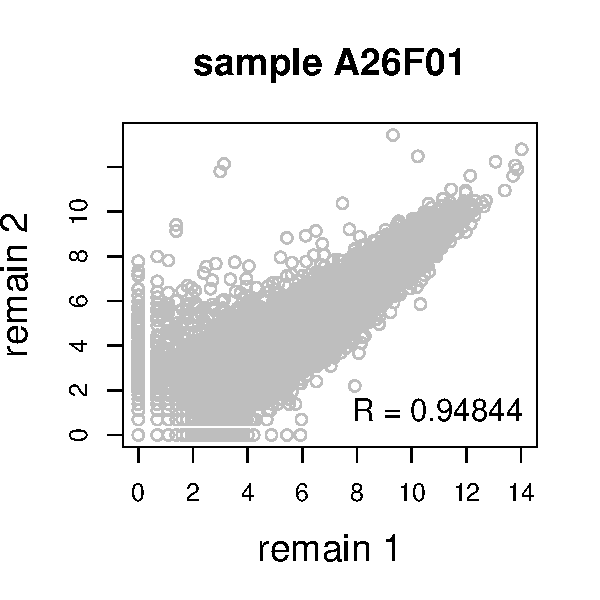
\includegraphics[width=0.3\textwidth]{Rep_picking_KeepKeep(5).pdf}
        }%
        \subcaptionbox{Remaining pair}{%
           \label{fig:rep_keepcut:A3OD}
           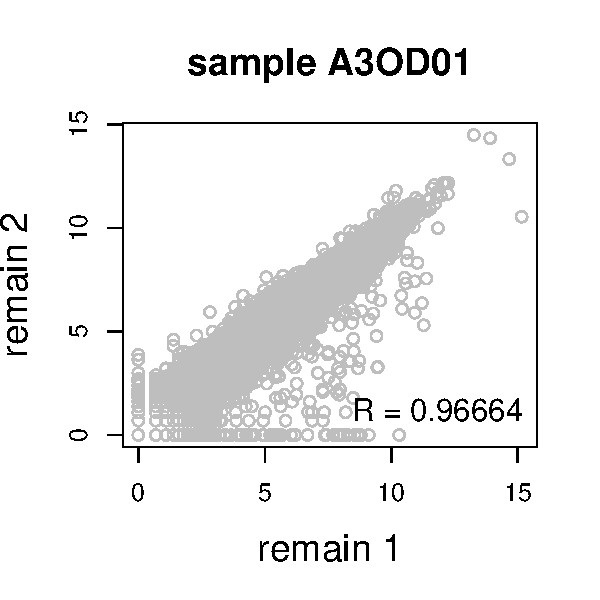
\includegraphics[width=0.3\textwidth]{Rep_picking_KeepKeep(6).pdf}
        }%
%
    \end{center}
    \caption[Replicate samples with all remaining]{\small \textbf{Replicate samples with all remaining.} Patient A26J was sampled 3 times and compared pairwise. Pairs of samples were also compared for other patients with replicate samples.  In all cases, replicate samples remaining in the dataset were highly concordant as shown by Pearson's correlation of log-raw counts.
}
\label{fig:rep_keepkeep}
%\end{mdframed}
\end{figure*}

\FloatBarrier

\begin{figure*}[!ht]
%\begin{mdframed}
           \begin{center}
%
        \subcaptionbox{Remaining}{%
           \label{fig:rep_keepcut:A0DB:first}
           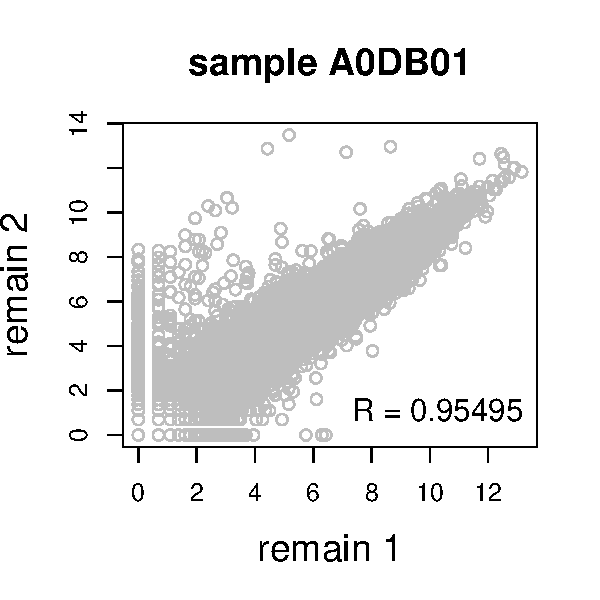
\includegraphics[width=0.3\textwidth]{Rep_picking_KeepCut(1).pdf}
        }%
        \subcaptionbox{Compare with excluded}{%
           \label{fig:rep_keepcut:A0DB:second}
           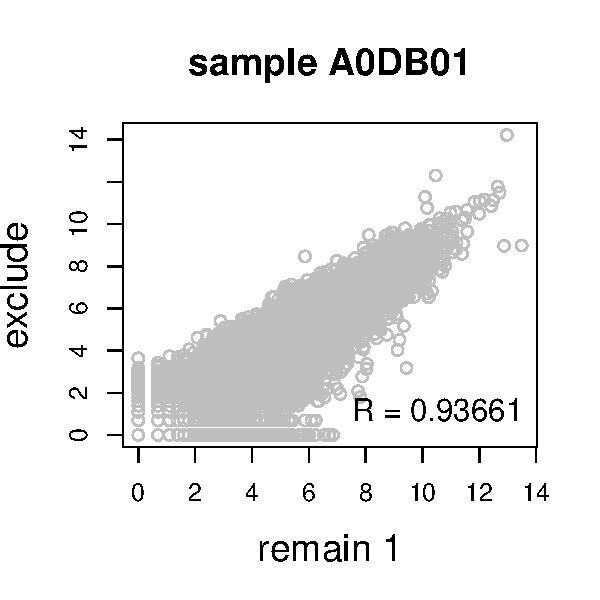
\includegraphics[width=0.3\textwidth]{Rep_picking_KeepCut(2).pdf}
        }%
        \subcaptionbox{Compare with excluded}{%
           \label{fig:rep_keepcut:A0DB:third}
           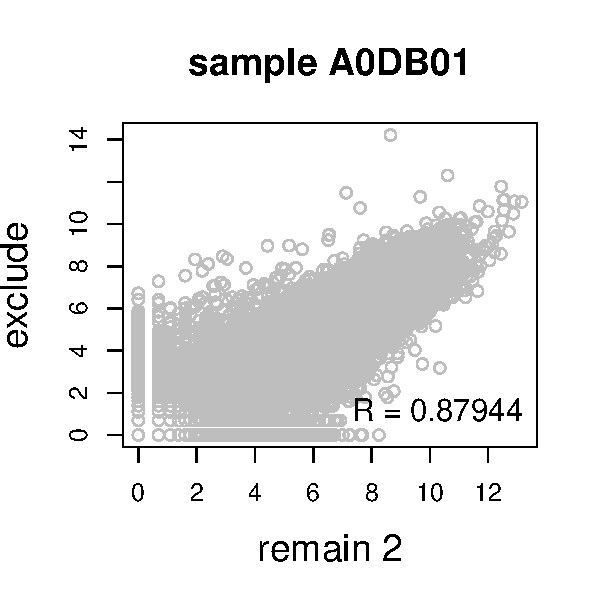
\includegraphics[width=0.3\textwidth]{Rep_picking_KeepCut(3).pdf}
        }%
%

%
        \subcaptionbox{Remaining}{%
           \label{fig:rep_keepcut:A13D:first}
           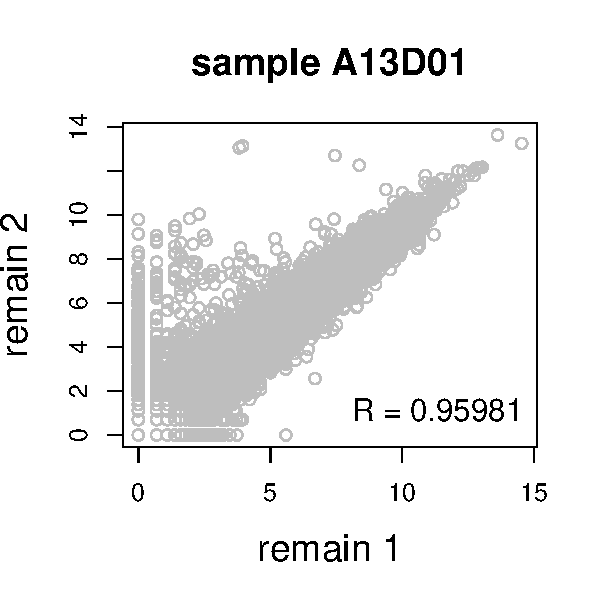
\includegraphics[width=0.3\textwidth]{Rep_picking_KeepCut(4).pdf}
        }%
        \subcaptionbox{Compare with excluded}{%
           \label{fig:rep_keepcut:A13D:second}
           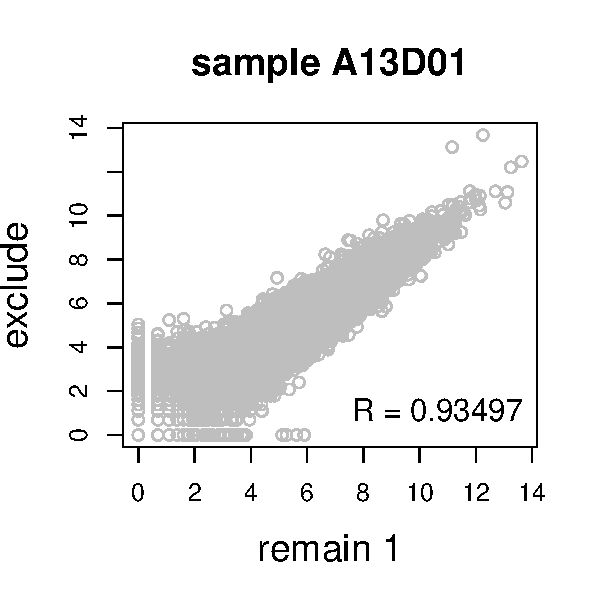
\includegraphics[width=0.3\textwidth]{Rep_picking_KeepCut(5).pdf}
        }%
        \subcaptionbox{Compare with excluded}{%
           \label{fig:rep_keepcut:A13D:third}
           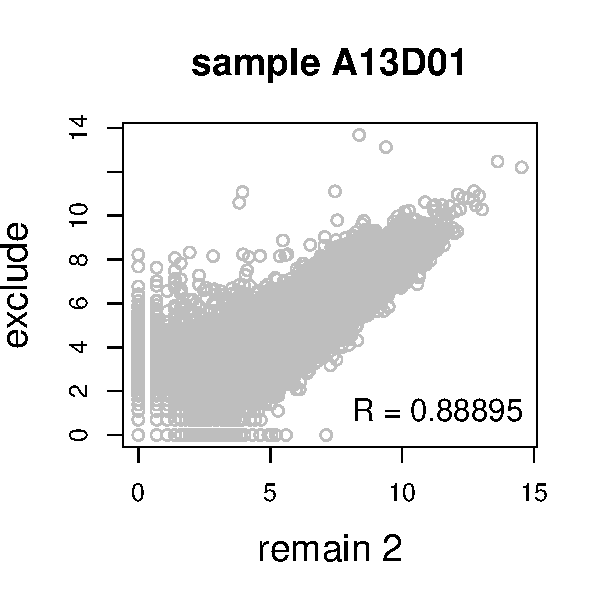
\includegraphics[width=0.3\textwidth]{Rep_picking_KeepCut(6).pdf}
        }%
%

%
        \subcaptionbox{Remaining}{%
           \label{fig:rep_keepcut:A13E:first}
           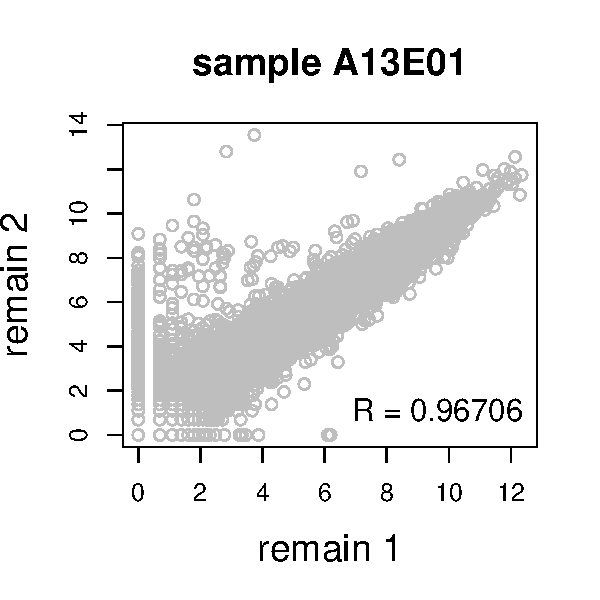
\includegraphics[width=0.3\textwidth]{Rep_picking_KeepCut(7).pdf}
        }%
        \subcaptionbox{Compare with excluded}{%
           \label{fig:rep_keepcut:A13E:second}
           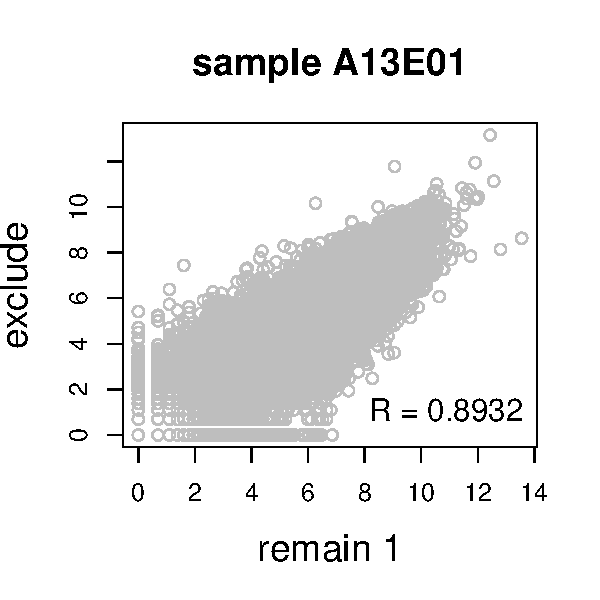
\includegraphics[width=0.3\textwidth]{Rep_picking_KeepCut(8).pdf}
        }%
        \subcaptionbox{Compare with excluded}{%
           \label{fig:rep_keepcut:A13E:third}
           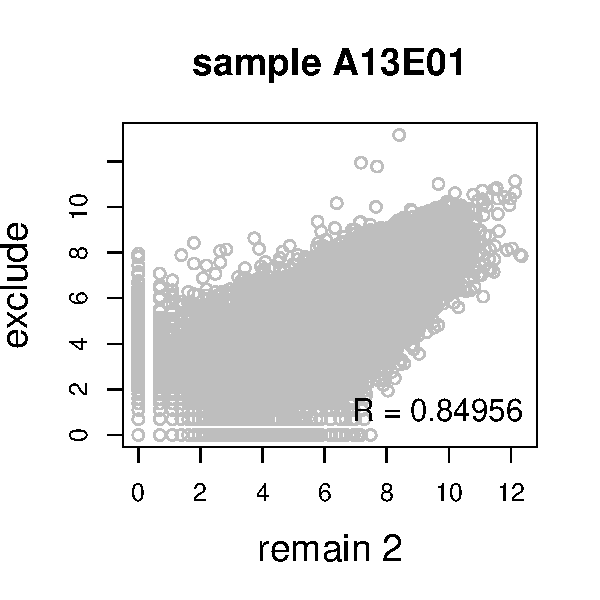
\includegraphics[width=0.3\textwidth]{Rep_picking_KeepCut(9).pdf}
        }%
%
    \end{center}
    \caption[Replicate samples with some excluded]{\small \textbf{Replicate samples with some excluded.} (continued on next page)
    %Patients A0DB, A13D, A13E, and A26E were each sampled 3 times and compared pairwise. Pairs of samples were also compared for other patients with replicate samples. In all cases, the replicate samples remaining in the dataset more were highly concordant (as shown by Pearson's correlation of log-raw counts) than those excluded from the analysis.
    }
%\end{mdframed}
\end{figure*}
\begin{figure*}[!ht]\ContinuedFloat
%\begin{mdframed}
     \begin{center}
%
        \subcaptionbox{Remaining}{%
           %\addtocounter{subfigure}{9}
           \label{fig:rep_keepcut:A26E:first}
           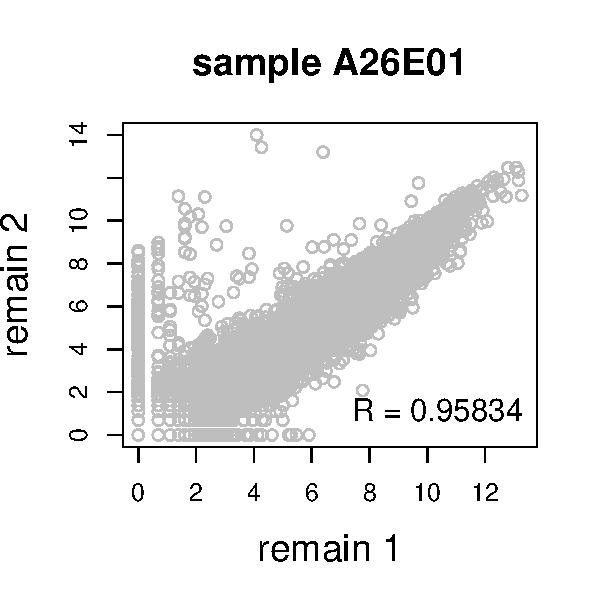
\includegraphics[width=0.3\textwidth]{Rep_picking_KeepCut(10).pdf}
        }%
        \subcaptionbox{Compare with excluded}{%
           \label{fig:rep_keepcut:A26E:second}
           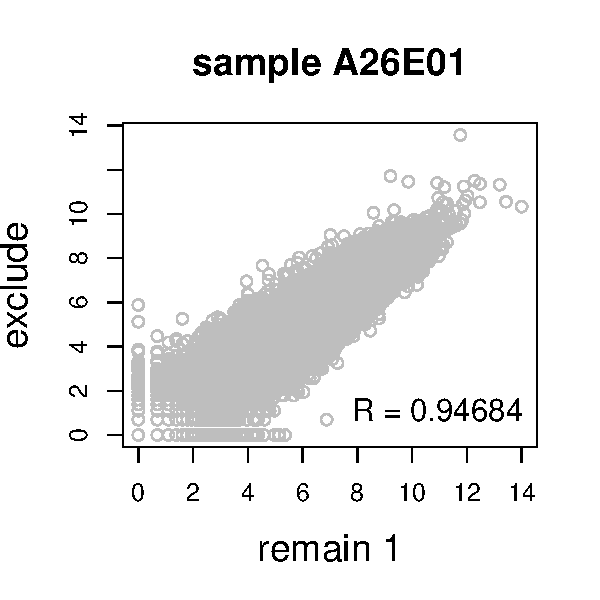
\includegraphics[width=0.3\textwidth]{Rep_picking_KeepCut(11).pdf}
        }%
        \subcaptionbox{Compare with excluded}{%
           \label{fig:rep_keepcut:A26E:third}
           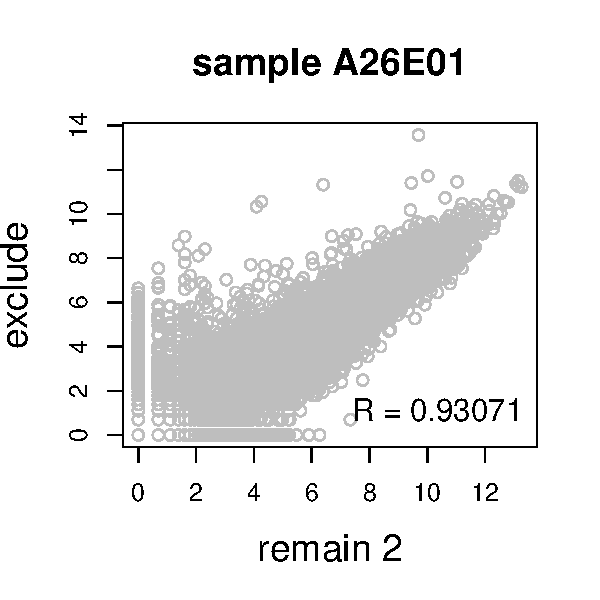
\includegraphics[width=0.3\textwidth]{Rep_picking_KeepCut(12).pdf}
        }%
%

%
        \subcaptionbox{Compare with excluded}{%
           \label{fig:rep_keepcut:A0DC}
           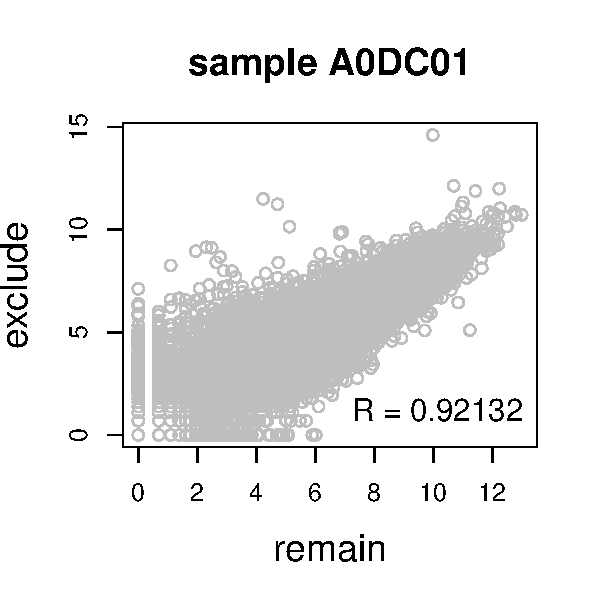
\includegraphics[width=0.3\textwidth]{Rep_picking_KeepCut(13).pdf}
        }%
        \subcaptionbox{Compare with excluded}{%
           \label{fig:rep_keepcut:A26I}
           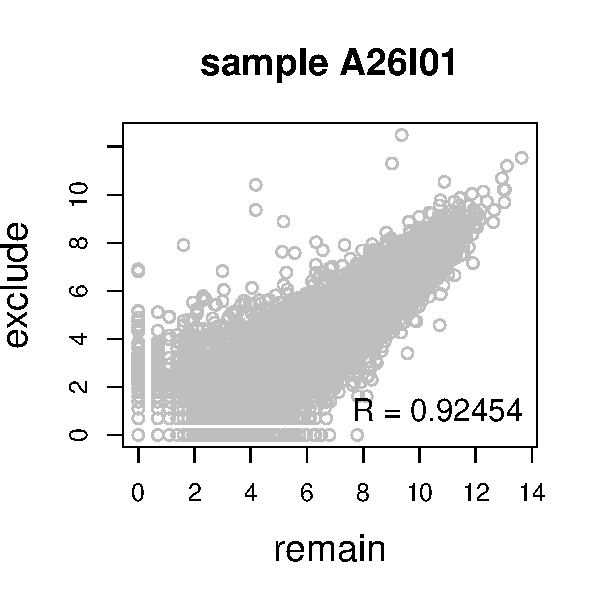
\includegraphics[width=0.3\textwidth]{Rep_picking_KeepCut(14).pdf}
        }%
%
    \end{center}
    \caption[]{\small \textbf{Replicate samples with some excluded.} Patients A0DB, A13D, A13E, and A26E were each sampled 3 times and compared pairwise. Pairs of samples were also compared for other patients with replicate samples. In all cases, the replicate samples remaining in the dataset more were highly concordant (as shown by Pearson's correlation of log-raw counts) than those excluded from the analysis.
}
\label{fig:rep_keepcut}
%\end{mdframed}
\end{figure*}


\chapter{Software Used for Thesis}
\label{appendix:software}

%centre longtable
\setlength{\LTleft}{-20cm plus -1fill}
\setlength{\LTright}{\LTleft}

%\makebox[\textwidth][c]{
%\resizebox{\textwidth}{!}{
\begin{longtable}{llllll}
\caption{R Packages used during Thesis}
\label{tab:computers_r_packages_full}
\\
\multicolumn{1}{l}{\bfseries Package}  & \multicolumn{1}{l}{\bfseries Repository}  & \multicolumn{1}{l}{\bfseries Laptop}      & \multicolumn{1}{l}{\bfseries Lab}         & \multicolumn{1}{l}{\bfseries Server}         & \multicolumn{1}{l}{\bfseries NeSI} \\ \hline \rowcolor{black!10}
base                          & base                      & 3.3.2       & 3.3.2       & 3.3.1          & 3.3.0             \\
%\hline
\rowcolor{black!5}
abind                         & CRAN                      &             & 1.4-5       &                & 1.4-3              \\
%\hline
\rowcolor{black!10}
acepack                       & CRAN                      &             & 1.4.1       &                & 1.3-3.3           \\
%\hline
\rowcolor{black!5}
ade4                          & CRAN                      &             & 1.7-5       &                &                    \\
%\hline
\rowcolor{black!10}
annaffy                       & Bioconductor              &             & 1.46.0      &                &                   \\
%\hline
\rowcolor{black!5}
AnnotationDbi                 & Bioconductor              &             & 1.36.0      & 1.36.0         & 1.34.4             \\
%\hline
\rowcolor{black!10}
apComplex                     & CRAN                      &             & 2.40.0      &                &                   \\
%\hline
\rowcolor{black!5}
ape                           & CRAN                      &             & 4           &                & 3.4                \\
%\hline
\rowcolor{black!10}
arm                           & CRAN                      &             & 1.9-3       &                &                   \\
%\hline
\rowcolor{black!5}
assertthat                    & CRAN                      & 0.1         & 0.1         & 0.1            & 0.1                \\
%\hline
\rowcolor{black!10}
backports                     & CRAN                      & 1.0.5       & 1.0.4       & 1.0.5          & 1.0.2             \\
%\hline
\rowcolor{black!5}
base64                        & CRAN                      &             &             & 2              & 2                  \\
%\hline
\rowcolor{black!10}
base64enc                     & CRAN                      &             & 0.1-3       &                & 0.1-3             \\
%\hline
\rowcolor{black!5}
beanplot                      & CRAN                      &             & 1.2         & 1.2            & 1.2                \\
%\hline
\rowcolor{black!10}
BH                            & CRAN                      & 1.60.0-2    & 1.62.0-1    & 1.62.0-1       & 1.60.0-2          \\
%\hline
\rowcolor{black!5}
Biobase                       & Bioconductor              &             & 2.34.0      & 2.34.0         & 2.32.0             \\
%\hline
\rowcolor{black!10}
BiocGenerics                  & Bioconductor              &             & 0.20.0      & 0.20.0         & 0.18.0            \\
%\hline
\rowcolor{black!5}
BiocInstaller                 & Bioconductor              &             & 1.24.0      & 1.20.3         & 1.22.3             \\
%\hline
\rowcolor{black!10}
BiocParallel                  & Bioconductor              &             & 1.8.1       & 1.8.1          &                   \\
%\hline
\rowcolor{black!5}
Biostrings                    & Bioconductor              &             & 2.42.1      & 2.42.0         &                    \\
%\hline
\rowcolor{black!10}
BiSEp                         & Bioconductor              &             & 2.0.1       & 2.0.1          & 2.0.1             \\
%\hline
\rowcolor{black!5}
bitops                        & CRAN                      & 1.0-6       & 1.0-6       & 1.0-6          & 1.0-6              \\
%\hline
\rowcolor{black!10}
boot                          & base                      & 1.3-18      & 1.3-18      & 1.3-18         & 1.3-18            \\
%\hline
\rowcolor{black!5}
brew                          & CRAN                      & 1.0-6       & 1.0-6       & 1.0-6          & 1.0-6              \\
%\hline
\rowcolor{black!10}
broom                         & CRAN                      & 0.4.1       &             &                &                   \\
%\hline
\rowcolor{black!5}
caTools                       & CRAN                      & 1.17.1      & 1.17.1      & 1.17.1         & 1.17.1             \\
%\hline
\rowcolor{black!10}
cgdsr                         & CRAN                      &             & 1.2.5       &                &                   \\
%\hline
\rowcolor{black!5}
checkmate                     & CRAN                      &             & 1.8.2       &                & 1.7.4              \\
%\hline
\rowcolor{black!10}
chron                         & CRAN                      & 2.3-47      & 2.3-48      & 2.3-50         & 2.3-47            \\
%\hline
\rowcolor{black!5}
class                         & base                      & 7.3-14      & 7.3-14      & 7.3-14         & 7.3-14             \\
%\hline
\rowcolor{black!10}
cluster                       & base                      & 2.0.5       & 2.0.5       & 2.0.5          & 2.0.4             \\
%\hline
\rowcolor{black!5}
coda                          & CRAN                      &             & 0.19-1      &                & 0.18-1             \\
%\hline
\rowcolor{black!10}
codetools                     & base                      & 0.2-15      & 0.2-15      & 0.2-15         & 0.2-14            \\
%\hline
\rowcolor{black!5}
colorRamps                    & CRAN                      &             & 2.3         &                &                    \\
%\hline
\rowcolor{black!10}
colorspace                    & CRAN                      & 1.2-6       & 1.3-2       & 1.3-2          & 1.2-6             \\
%\hline
\rowcolor{black!5}
commonmark                    & CRAN                      & 1.1         &             & 1.2            &                    \\
%\hline
\rowcolor{black!10}
compiler                      & base                      & 3.3.2       & 3.3.2       & 3.3.1          & 3.3.0             \\
%\hline
\rowcolor{black!5}
corpcor                       & CRAN                      &             & 1.6.8       & 1.6.8          & 1.6.8              \\
%\hline
\rowcolor{black!10}
Cprob                         & CRAN                      &             & 1.2.4       &                &                   \\
%\hline
\rowcolor{black!5}
crayon                        & CRAN                      & 1.3.2       & 1.3.2       & 1.3.2          & 1.3.2              \\
%\hline
\rowcolor{black!10}
crop                          & CRAN                      &             & 0.0-2       & 0.0-2          &                   \\
%\hline
\rowcolor{black!5}
curl                          & CRAN                      & 1.2         & 2.3         & 2.3            & 0.9.7              \\
%\hline
\rowcolor{black!10}
d3Network                     & CRAN                      &             & 0.5.2.1     &                &                   \\
%\hline
\rowcolor{black!5}
data.table                    & CRAN                      & 1.9.6       & 1.10.0      & 1.10.1         & 1.9.6              \\
%\hline
\rowcolor{black!10}
data.tree                     & CRAN                      &             & 0.7.0       & 0.7.0          &                   \\
%\hline
\rowcolor{black!5}
datasets                      & base                      & 3.3.2       & 3.3.2       & 3.3.1          & 3.3.0              \\
%\hline
\rowcolor{black!10}
DBI                           & CRAN                      & 0.5-1       & 0.5-1       & 0.5-1          & 0.5-1             \\
%\hline
\rowcolor{black!5}
dendextend                    & CRAN                      & 1.4.0       & 1.4.0       & 1.4.0          &                    \\
%\hline
\rowcolor{black!10}
DEoptimR                      & CRAN                      & 1.0-8       & 1.0-8       & 1.0-8          & 1.0-4             \\
%\hline
\rowcolor{black!5}
desc                          & CRAN                      & 1.1.0       &             & 1.1.0          &                    \\
%\hline
\rowcolor{black!10}
devtools                      & CRAN                      & 1.12.0      & 1.12.0      & 1.12.0         & 1.12.0            \\
%\hline
\rowcolor{black!5}
DiagrammeR                    & CRAN                      &             & 0.9.0       & 0.9.0          &                    \\
%\hline
\rowcolor{black!10}
dichromat                     & CRAN                      & 2.0-0       & 2.0-0       & 2.0-0          & 2.0-0             \\
%\hline
\rowcolor{black!5}
digest                        & CRAN                      & 0.6.10      & 0.6.11      & 0.6.12         & 0.6.9              \\
%\hline
\rowcolor{black!10}
diptest                       & CRAN                      & 0.75-7      & 0.75-7      & 0.75-7         &                   \\
%\hline
\rowcolor{black!5}
doParallel                    & CRAN                      & 1.0.10      & 1.0.10      & 1.0.10         & 1.0.10             \\
%\hline
\rowcolor{black!10}
dplyr                         & CRAN                      & 0.5.0       & 0.5.0       & 0.5.0          & 0.5.0             \\
%\hline
\rowcolor{black!5}
ellipse                       & CRAN                      &             & 0.3-8       & 0.3-8          & 0.3-8              \\
%\hline
\rowcolor{black!10}
evaluate                      & CRAN                      &             & 0.1         & 0.1            & 0.9               \\
%\hline
\rowcolor{black!5}
fdrtool                       & CRAN                      &             & 1.2.15      &                &                    \\
%\hline
\rowcolor{black!10}
fields                        & CRAN                      &             & 8.1         &                &                   \\
%\hline
\rowcolor{black!5}
flexmix                       & CRAN                      & 2.3-13      & 2.3-13      & 2.3-13         &                    \\
%\hline
\rowcolor{black!10}
forcats                       & CRAN                      & 0.2.0       &             &                &                   \\
%\hline
\rowcolor{black!5}
foreach                       & CRAN                      & 1.4.3       & 1.4.3       & 1.4.3          & 1.4.3              \\
%\hline
\rowcolor{black!10}
foreign                       & base                      & 0.8-67      & 0.8-67      & 0.8-67         & 0.8-66            \\
%\hline
\rowcolor{black!5}
formatR                       & CRAN                      &             & 1.4         & 1.4            & 1.4                \\
%\hline
\rowcolor{black!10}
Formula                       & CRAN                      &             & 1.2-1       &                & 1.2-1             \\
%\hline
\rowcolor{black!5}
fpc                           & CRAN                      & 2.1-10      & 2.1-10      & 2.1-10         &                    \\
%\hline
\rowcolor{black!10}
futile.logger                 & CRAN                      &             & 1.4.3       & 1.4.3          & 1.4.1             \\
%\hline
\rowcolor{black!5}
futile.options                & CRAN                      &             & 1.0.0       & 1.0.0          & 1.0.0              \\
%\hline
\rowcolor{black!10}
gdata                         & CRAN                      & 2.17.0      & 2.17.0      & 2.17.0         & 2.17.0            \\
%\hline
\rowcolor{black!5}
geepack                       & CRAN                      &             & 1.2-1       &                &                    \\
%\hline
\rowcolor{black!10}
GenomeInfoDb                  & Bioconductor              &             & 1.10.2      & 1.10.1         &                   \\
%\hline
\rowcolor{black!5}
GenomicAlignments             & Bioconductor              &             & 1.10.0      & 1.10.0         &                    \\
%\hline
\rowcolor{black!10}
GenomicRanges                 & Bioconductor              &             & 1.26.2      & 1.26.1         &                   \\
%\hline
\rowcolor{black!5}
ggm                           & CRAN                      &             & 2.3         &                &                    \\
%\hline
\rowcolor{black!10}
ggplot2                       & CRAN                      & 2.1.0       & 2.2.1       & 2.2.1          & 2.1.0             \\
%\hline
\rowcolor{black!5}
git2r                         & CRAN                      & 0.15.0      & 0.18.0      & 0.16.0         & 0.15.0             \\
%\hline
\rowcolor{black!10}
glasso                        & CRAN                      &             & 1.8         &                &                   \\
%\hline
\rowcolor{black!5}
GO.db                         & Bioconductor              &             & 3.4.0       & 3.2.2          & 3.3.0              \\
%\hline
\rowcolor{black!10}
GOSemSim                      & Bioconductor              &             & 2.0.3       & 1.28.2         & 1.30.3            \\
%\hline
\rowcolor{black!5}
gplots                        & CRAN                      & 3.0.1       & 3.0.1       & 3.0.1          & 3.0.1              \\
%\hline
\rowcolor{black!10}
graph                         & Bioconductor              &             & 1.52.0      &                &                   \\
%\hline
\rowcolor{black!5}
graphics                      & base                      & 3.3.2       & 3.3.2       & 3.3.1          & 3.3.0              \\
%\hline
\rowcolor{black!10}
graphsim                      & \begin{tabular}[c]{@{}l@{}}GitHub \\ TomKellyGenetics \end{tabular}  & 0.1.0       & 0.1.0       & 0.1.0          & 0.1.0             \\
%\hline
\rowcolor{black!5}
grDevices                     & base                      & 3.3.2       & 3.3.2       & 3.3.1          & 3.3.0              \\
%\hline
\rowcolor{black!10}
grid                          & base                      & 3.3.2       & 3.3.2       & 3.3.1          & 3.3.0             \\
%\hline
\rowcolor{black!5}
gridBase                      & CRAN                      & 0.4-7       & 0.4-7       & 0.4-7          & 0.4-7              \\
%\hline
\rowcolor{black!10}
gridExtra                     & CRAN                      & 2.2.1       & 2.2.1       & 2.2.1          & 2.2.1             \\
%\hline
\rowcolor{black!5}
gridGraphics                  & CRAN                      &             & 0.1-5       &                &                    \\
%\hline
\rowcolor{black!10}
gtable                        & CRAN                      & 0.2.0       & 0.2.0       & 0.2.0          & 0.2.0             \\
%\hline
\rowcolor{black!5}
gtools                        & CRAN                      & 3.5.0       & 3.5.0       & 3.5.0          & 3.5.0              \\
%\hline
\rowcolor{black!10}
haven                         & CRAN                      & 1.0.0       &             &                &                   \\
%\hline
\rowcolor{black!5}
heatmap.2x                    & \begin{tabular}[c]{@{}l@{}}GitHub \\ TomKellyGenetics \end{tabular}  & 0.0.0.9000  & 0.0.0.9000  & 0.0.0.9000     & 0.0.0.9000         \\
%\hline
\rowcolor{black!10}
hgu133plus2.db                & Bioconductor              &             & 3.2.3       &                &                   \\
%\hline
\rowcolor{black!5}
highr                         & CRAN                      &             & 0.6         & 0.6            & 0.6                \\
%\hline
\rowcolor{black!10}
Hmisc                         & CRAN                      &             & 4.0-2       & 4.0-2          & 3.17-4            \\
%\hline
\rowcolor{black!5}
hms                           & CRAN                      & 0.2         & 0.3         &                &                    \\
%\hline
\rowcolor{black!10}
htmlTable                     & CRAN                      &             & 1.8         & 1.9            &                   \\
%\hline
\rowcolor{black!5}
htmltools                     & CRAN                      & 0.3.5       & 0.3.5       & 0.3.5          & 0.3.5              \\
%\hline
\rowcolor{black!10}
htmlwidgets                   & CRAN                      &             & 0.8         & 0.8            &                   \\
%\hline
\rowcolor{black!5}
httpuv                        & CRAN                      & 1.3.3       &             & 1.3.3          &                    \\
%\hline
\rowcolor{black!10}
httr                          & CRAN                      & 1.2.1       & 1.2.1       & 1.2.1          & 1.1.0             \\
%\hline
\rowcolor{black!5}
huge                          & CRAN                      &             & 1.2.7       &                &                    \\
%\hline
\rowcolor{black!10}
hunspell                      & CRAN                      &             & 2.3         &                & 2                 \\
%\hline
\rowcolor{black!5}
hypergraph                    & CRAN                      &             & 1.46.0      &                &                    \\
%\hline
\rowcolor{black!10}
igraph                        & CRAN                      & 1.0.1       & 1.0.1       & 1.0.1          & 1.0.1             \\
%\hline
\rowcolor{black!5}
igraph.extensions             & \begin{tabular}[c]{@{}l@{}}GitHub \\ TomKellyGenetics \end{tabular}  & 0.1.0.9001  & 0.1.0.9001  & 0.1.0.9001     & 0.1.0.9001         \\
%\hline
\rowcolor{black!10}
influenceR                    & CRAN                      &             & 0.1.0       & 0.1.0          &                   \\
%\hline
\rowcolor{black!5}
info.centrality               & \begin{tabular}[c]{@{}l@{}}GitHub \\ TomKellyGenetics \end{tabular}  & 0.1.0       & 0.1.0       & 0.1.0          & 0.1.0              \\
%\hline
\rowcolor{black!10}
IRanges                       & Bioconductor              &             & 2.8.1       & 2.8.1          & 2.6.1             \\
%\hline
\rowcolor{black!5}
irlba                         & CRAN                      & 2.1.1       & 2.1.2       & 2.1.2          & 2.0.0              \\
%\hline
\rowcolor{black!10}
iterators                     & CRAN                      & 1.0.8       & 1.0.8       & 1.0.8          & 1.0.8             \\
%\hline
\rowcolor{black!5}
jpeg                          & CRAN                      &             & 0.1-8       &                &                    \\
%\hline
\rowcolor{black!10}
jsonlite                      & CRAN                      & 1.1         & 1.2         & 1.3            & 0.9.20            \\
%\hline
\rowcolor{black!5}
KEGG.db                       & Bioconductor              &             & 3.2.3       &                &                    \\
%\hline
\rowcolor{black!10}
kernlab                       & CRAN                      & 0.9-25      & 0.9-25      & 0.9-25         &                   \\
%\hline
\rowcolor{black!5}
KernSmooth                    & base                      & 2.23-15     & 2.23-15     & 2.23-15        & 2.23-15            \\
%\hline
\rowcolor{black!10}
knitr                         & CRAN                      &             & 1.15.1      & 1.15.1         & 1.14              \\
%\hline
\rowcolor{black!5}
labeling                      & CRAN                      & 0.3         & 0.3         & 0.3            & 0.3                \\
%\hline
\rowcolor{black!10}
lambda.r                      & CRAN                      &             & 1.1.9       & 1.1.9          & 1.1.7             \\
%\hline
\rowcolor{black!5}
lattice                       & base                      & 0.20-34     & 0.20-34     & 0.20-34        & 0.20-33            \\
%\hline
\rowcolor{black!10}
latticeExtra                  & CRAN                      &             & 0.6-28      &                & 0.6-28            \\
%\hline
\rowcolor{black!5}
lava                          & CRAN                      &             & 1.4.6       &                &                    \\
%\hline
\rowcolor{black!10}
lavaan                        & CRAN                      &             & 0.5-22      &                &                   \\
%\hline
\rowcolor{black!5}
lazyeval                      & CRAN                      & 0.2.0       & 0.2.0       & 0.2.0          & 0.2.0              \\
%\hline
\rowcolor{black!10}
les                           & CRAN                      &             & 1.24.0      &                &                   \\
%\hline
\rowcolor{black!5}
lgtdl                         & CRAN                      &             & 1.1.3       &                &                    \\
%\hline
\rowcolor{black!10}
limma                         & Bioconductor              &             & 3.30.7      & 3.30.3         &                   \\
%\hline
\rowcolor{black!5}
lme4                          & CRAN                      &             & 1.1-12      &                & 1.1-12             \\
%\hline
\rowcolor{black!10}
lubridate                     & CRAN                      & 1.6.0       &             &                &                   \\
%\hline
\rowcolor{black!5}
magrittr                      & CRAN                      & 1.5         & 1.5         & 1.5            & 1.5                \\
%\hline
\rowcolor{black!10}
maps                          & CRAN                      &             & 3.1.1       &                &                   \\
%\hline
\rowcolor{black!5}
markdown                      & CRAN                      &             & 0.7.7       & 0.7.7          & 0.7.7              \\
%\hline
\rowcolor{black!10}
MASS                          & base                      & 7.3-45      & 7.3-45      & 7.3-45         & 7.3-45            \\
%\hline
\rowcolor{black!5}
Matrix                        & base                      & 1.2-7.1     & 1.2-7.1     & 1.2-8          & 1.2-6              \\
%\hline
\rowcolor{black!10}
matrixcalc                    & CRAN                      & 1.0-3       & 1.0-3       & 1.0-3          & 1.0-3             \\
%\hline
\rowcolor{black!5}
mclust                        & CRAN                      & 5.2         & 5.2.1       & 5.2.2          & 5.2                \\
%\hline
\rowcolor{black!10}
memoise                       & CRAN                      & 1.0.0       & 1.0.0       & 1.0.0          & 1.0.0             \\
%\hline
\rowcolor{black!5}
methods                       & base                      & 3.3.2       & 3.3.2       & 3.3.1          & 3.3.0              \\
%\hline
\rowcolor{black!10}
mgcv                          & base                      & 1.8-16      & 1.8-16      & 1.8-17         & 1.8-12            \\
%\hline
\rowcolor{black!5}
mi                            & CRAN                      &             & 1           &                &                    \\
%\hline
\rowcolor{black!10}
mime                          & CRAN                      & 0.5         & 0.5         & 0.5            & 0.4               \\
%\hline
\rowcolor{black!5}
minqa                         & CRAN                      &             & 1.2.4       &                & 1.2.4              \\
%\hline
\rowcolor{black!10}
mnormt                        & CRAN                      & 1.5-5       & 1.5-5       &                & 1.5-4             \\
%\hline
\rowcolor{black!5}
modelr                        & CRAN                      & 0.1.0       &             &                &                    \\
%\hline
\rowcolor{black!10}
modeltools                    & CRAN                      & 0.2-21      & 0.2-21      & 0.2-21         &                   \\
%\hline
\rowcolor{black!5}
multtest                      & Bioconductor              &             & 2.30.0      & 2.30.0         &                    \\
%\hline
\rowcolor{black!10}
munsell                       & CRAN                      & 0.4.3       & 0.4.3       & 0.4.3          & 0.4.3             \\
%\hline
\rowcolor{black!5}
mvtnorm                       & CRAN                      & 1.0-5       & 1.0-5       & 1.0-6          & 1.0-5              \\
%\hline
\rowcolor{black!10}
network                       & CRAN                      &             & 1.13.0      &                &                   \\
%\hline
\rowcolor{black!5}
nlme                          & base                      & 3.1-128     & 3.1-128     & 3.1-131        & 3.1-128            \\
%\hline
\rowcolor{black!10}
nloptr                        & CRAN                      &             & 1.0.4       &                & 1.0.4             \\
%\hline
\rowcolor{black!5}
NMF                           & CRAN                      & 0.20.6      & 0.20.6      & 0.20.6         & 0.20.6             \\
%\hline
\rowcolor{black!10}
nnet                          & base                      & 7.3-12      & 7.3-12      & 7.3-12         & 7.3-12            \\
%\hline
\rowcolor{black!5}
numDeriv                      & CRAN                      &             & 2016.8-1    &                & 2014.2-1           \\
%\hline
\rowcolor{black!10}
openssl                       & CRAN                      & 0.9.4       & 0.9.6       & 0.9.6          & 0.9.4             \\
%\hline
\rowcolor{black!5}
org.Hs.eg.db                  & Bioconductor              &             & 3.1.2       &                & 3.3.0              \\
%\hline
\rowcolor{black!10}
org.Sc.sgd.db                 & Bioconductor              &             & 3.4.0       &                &                   \\
%\hline
\rowcolor{black!5}
parallel                      & base                      & 3.3.2       & 3.3.2       & 3.3.1          & 3.3.0              \\
%\hline
\rowcolor{black!10}
\begin{tabular}[c]{@{}l@{}}pathway.structure\\.permutation \end{tabular} & \begin{tabular}[c]{@{}l@{}}GitHub \\ TomKellyGenetics \end{tabular}  & 0.1.0       & 0.1.0       & 0.1.0          & 0.1.0             \\
%\hline
\rowcolor{black!5}
pbivnorm                      & CRAN                      &             & 0.6.0       &                &                    \\
%\hline
\rowcolor{black!10}
PGSEA                         & Bioconductor              &             & 1.48.0      &                &                   \\
%\hline
\rowcolor{black!5}
pkgmaker                      & CRAN                      & 0.22        & 0.22        & 0.22           & 0.22               \\
%\hline
\rowcolor{black!10}
PKI                           & CRAN                      &             & 0.1-3       &                &                   \\
%\hline
\rowcolor{black!5}
plogr                         & CRAN                      &             & 0.1-1       & 0.1-1          &                    \\
%\hline
\rowcolor{black!10}
plot.igraph                   & \begin{tabular}[c]{@{}l@{}}GitHub \\ TomKellyGenetics \end{tabular}  & 0.0.0.9001  & 0.0.0.9001  & 0.0.0.9001     & 0.0.0.9001        \\
%\hline
\rowcolor{black!5}
plotrix                       & CRAN                      &             & 3.6-4       &                &                    \\
%\hline
\rowcolor{black!10}
plyr                          & CRAN                      & 1.8.4       & 1.8.4       & 1.8.4          & 1.8.3             \\
%\hline
\rowcolor{black!5}
png                           & CRAN                      &             & 0.1-7       &                & 0.1-7              \\
%\hline
\rowcolor{black!10}
prabclus                      & CRAN                      & 2.2-6       & 2.2-6       & 2.2-6          &                   \\
%\hline
\rowcolor{black!5}
praise                        & CRAN                      & 1.0.0       & 1.0.0       &                & 1.0.0              \\
%\hline
\rowcolor{black!10}
pROC                          & CRAN                      &             & 1.8         & 1.9.1          &                   \\
%\hline
\rowcolor{black!5}
prodlim                       & CRAN                      &             & 1.5.7       &                &                    \\
%\hline
\rowcolor{black!10}
prof.tree                     & CRAN                      &             & 0.1.0       &                &                   \\
%\hline
\rowcolor{black!5}
proftools                     & CRAN                      &             & 0.99-2      &                &                    \\
%\hline
\rowcolor{black!10}
progress                      & CRAN                      &             &             & 1.1.2          &                   \\
%\hline
\rowcolor{black!5}
psych                         & CRAN                      & 1.6.12      & 1.6.12      &                &                    \\
%\hline
\rowcolor{black!10}
purrr                         & CRAN                      & 0.2.2       & 0.2.2       & 0.2.2          & 0.2.2             \\
%\hline
\rowcolor{black!5}
qgraph                        & CRAN                      &             & 1.4.1       &                &                    \\
%\hline
\rowcolor{black!10}
quadprog                      & CRAN                      &             & 1.5-5       & 1.5-5          & 1.5-5             \\
%\hline
\rowcolor{black!5}
R.methodsS3                   & CRAN                      &             & 1.7.1       &                & 1.7.1              \\
%\hline
\rowcolor{black!10}
R.oo                          & CRAN                      &             & 1.21.0      &                & 1.20.0            \\
%\hline
\rowcolor{black!5}
R.utils                       & CRAN                      &             & 2.5.0       &                &                    \\
%\hline
\rowcolor{black!10}
R6                            & CRAN                      & 2.1.3       & 2.2.0       & 2.2.0          & 2.1.3             \\
%\hline
\rowcolor{black!5}
RBGL                          & CRAN                      &             & 1.50.0      &                &                    \\
%\hline
\rowcolor{black!10}
RColorBrewer                  & CRAN                      & 1.1-2       & 1.1-2       & 1.1-2          & 1.1-2             \\
%\hline
\rowcolor{black!5}
Rcpp                          & CRAN                      & 0.12.7      & 0.12.9      & 0.12.9         & 0.12.7             \\
%\hline
\rowcolor{black!10}
RcppArmadillo                 & CRAN                      &             &             & 0.7.700.0.0    & 0.6.700.6.0       \\
%\hline
\rowcolor{black!5}
RcppEigen                     & CRAN                      &             & 0.3.2.9.0   &                & 0.3.2.8.1          \\
%\hline
\rowcolor{black!10}
RCurl                         & CRAN                      &             & 1.95-4.8    & 1.95-4.8       & 1.95-4.8          \\
%\hline
\rowcolor{black!5}
reactome.db                   & Bioconductor              &             & 1.52.1      & 1.52.1         &                    \\
%\hline
\rowcolor{black!10}
reactometree                  & \begin{tabular}[c]{@{}l@{}}GitHub \\ TomKellyGenetics \end{tabular}  &             & 0.1         &                &                   \\
%\hline
\rowcolor{black!5}
readr                         & CRAN                      & 1.0.0       & 1.0.0       &                &                    \\
%\hline
\rowcolor{black!10}
readxl                        & CRAN                      & 0.1.1       &             &                &                   \\
%\hline
\rowcolor{black!5}
registry                      & CRAN                      & 0.3         & 0.3         & 0.3            & 0.3                \\
%\hline
\rowcolor{black!10}
reshape2                      & CRAN                      & 1.4.1       & 1.4.2       & 1.4.2          & 1.4.1             \\
%\hline
\rowcolor{black!5}
rgexf                         & CRAN                      &             & 0.15.3      & 0.15.3         &                    \\
%\hline
\rowcolor{black!10}
rgl                           & CRAN                      &             &             & 0.97.0         & 0.95.1441         \\
%\hline
\rowcolor{black!5}
Rgraphviz                     & CRAN                      &             & 2.18.0      &                &                    \\
%\hline
\rowcolor{black!10}
rjson                         & CRAN                      &             & 0.2.15      &                &                   \\
%\hline
\rowcolor{black!5}
RJSONIO                       & CRAN                      &             & 1.3-0       &                &                    \\
%\hline
\rowcolor{black!10}
rmarkdown                     & CRAN                      &             & 1.3         & 1.3            & 1                 \\
%\hline
\rowcolor{black!5}
Rmpi                          & CRAN                      &             & 0.6-6       &                & 0.6-5              \\
%\hline
\rowcolor{black!10}
rngtools                      & CRAN                      & 1.2.4       & 1.2.4       & 1.2.4          & 1.2.4             \\
%\hline
\rowcolor{black!5}
robustbase                    & CRAN                      & 0.92-7      & 0.92-7      & 0.92-7         & 0.92-5             \\
%\hline
\rowcolor{black!10}
ROCR                          & CRAN                      & 1.0-7       & 1.0-7       & 1.0-7          & 1.0-7             \\
%\hline
\rowcolor{black!5}
Rook                          & CRAN                      &             & 1.1-1       & 1.1-1          &                    \\
%\hline
\rowcolor{black!10}
roxygen2                      & CRAN                      & 6.0.1       & 5.0.1       & 6.0.1          & 5.0.1             \\
%\hline
\rowcolor{black!5}
rpart                         & base                      & 4.1-10      & 4.1-10      & 4.1-10         & 4.1-10             \\
%\hline
\rowcolor{black!10}
rprojroot                     & CRAN                      & 1.2         & 1.1         & 1.2            &                   \\
%\hline
\rowcolor{black!5}
Rsamtools                     & Bioconductor              &             & 1.26.1      & 1.26.1         &                    \\
%\hline
\rowcolor{black!10}
rsconnect                     & CRAN                      &             & 0.7         &                &                   \\
%\hline
\rowcolor{black!5}
RSQLite                       & CRAN                      &             & 1.1-2       & 1.1-2          & 1.0.0              \\
%\hline
\rowcolor{black!10}
rstudioapi                    & CRAN                      & 0.6         & 0.6         & 0.6            & 0.6               \\
%\hline
\rowcolor{black!5}
rvest                         & CRAN                      & 0.3.2       &             &                &                    \\
%\hline
\rowcolor{black!10}
S4Vectors                     & Bioconductor              &             & 0.12.1      & 0.12.0         & 0.10.3            \\
%\hline
\rowcolor{black!5}
safe                          & Bioconductor              &             & 3.14.0      & 3.10.0         &                    \\
%\hline
\rowcolor{black!10}
scales                        & CRAN                      & 0.4.0       & 0.4.1       & 0.4.1          & 0.4.0             \\
%\hline
\rowcolor{black!5}
selectr                       & CRAN                      & 0.3-1       &             &                &                    \\
%\hline
\rowcolor{black!10}
sem                           & CRAN                      &             & 3.1-8       &                &                   \\
%\hline
\rowcolor{black!5}
shiny                         & CRAN                      & 0.14        &             & 1.0.0          &                    \\
%\hline
\rowcolor{black!10}
slipt                         & \begin{tabular}[c]{@{}l@{}}GitHub \\ TomKellyGenetics \end{tabular}  & 0.1.0       & 0.1.0       & 0.1.0          & 0.1.0             \\
%\hline
\rowcolor{black!5}
sm                            & CRAN                      & 2.2-5.4     & 2.2-5.4     &                &                    \\
%\hline
\rowcolor{black!10}
sna                           & CRAN                      &             & 2.4         &                &                   \\
%\hline
\rowcolor{black!5}
snow                          & CRAN                      & 0.4-1       & 0.4-2       & 0.4-2          & 0.3-13             \\
%\hline
\rowcolor{black!10}
sourcetools                   & CRAN                      & 0.1.5       &             & 0.1.5          &                   \\
%\hline
\rowcolor{black!5}
SparseM                       & CRAN                      &             & 1.74        &                & 1.7                \\
%\hline
\rowcolor{black!10}
spatial                       & base                      & 7.3-11      & 7.3-11      & 7.3-11         & 7.3-11            \\
%\hline
\rowcolor{black!5}
splines                       & base                      & 3.3.2       & 3.3.2       & 3.3.1          & 3.3.0              \\
%\hline
\rowcolor{black!10}
statnet.common                & CRAN                      &             & 3.3.0       &                &                   \\
%\hline
\rowcolor{black!5}
stats                         & base                      & 3.3.2       & 3.3.2       & 3.3.1          & 3.3.0              \\
%\hline
\rowcolor{black!10}
stats4                        & base                      & 3.3.2       & 3.3.2       & 3.3.1          & 3.3.0             \\
%\hline
\rowcolor{black!5}
stringi                       & CRAN                      & 1.1.1       & 1.1.2       & 1.1.2          & 1.0-1              \\
%\hline
\rowcolor{black!10}
stringr                       & CRAN                      & 1.1.0       & 1.1.0       & 1.2.0          & 1.0.0             \\
%\hline
\rowcolor{black!5}
\begin{tabular}[c]{@{}l@{}}Summarized\\Experiment \end{tabular}          & Bioconductor              &             & 1.4.0       & 1.4.0          &                    \\
%\hline
\rowcolor{black!10}
survival                      & base                      & 2.39-4      & 2.40-1      & 2.40-1         & 2.39-4            \\
%\hline
\rowcolor{black!5}
tcltk                         & base                      & 3.3.2       & 3.3.2       & 3.3.1          & 3.3.0              \\
%\hline
\rowcolor{black!10}
testthat                      & CRAN                      & 1.0.2       & 1.0.2       &                & 1.0.2             \\
%\hline
\rowcolor{black!5}
tibble                        & CRAN                      & 1.2         & 1.2         & 1.2            & 1.2                \\
%\hline
\rowcolor{black!10}
tidyr                         & CRAN                      & 0.6.1       & 0.6.1       & 0.6.1          &                   \\
%\hline
\rowcolor{black!5}
tidyverse                     & \begin{tabular}[c]{@{}l@{}}GitHub \\ hadley \end{tabular}            & 1.1.1       &             &                &                    \\
%\hline
\rowcolor{black!10}
timeline                      & CRAN                      &             & 0.9         &                &                   \\
%\hline
\rowcolor{black!5}
tools                         & base                      & 3.3.2       & 3.3.2       & 3.3.1          & 3.3.0              \\
%\hline
\rowcolor{black!10}
tpr                           & CRAN                      &             & 0.3-1       &                &                   \\
%\hline
\rowcolor{black!5}
trimcluster                   & CRAN                      & 0.1-2       & 0.1-2       & 0.1-2          &                    \\
%\hline
\rowcolor{black!10}
Unicode                       & CRAN                      & 9.0.0-1     & 9.0.0-1     & 9.0.0-1        &                   \\
%\hline
\rowcolor{black!5}
utils                         & base                      & 3.3.2       & 3.3.2       & 3.3.1          & 3.3.0              \\
%\hline
\rowcolor{black!10}
vioplot                       & CRAN                      &             & 0.2         &                &                   \\
%\hline
\rowcolor{black!5}
vioplotx                      & \begin{tabular}[c]{@{}l@{}}GitHub \\ TomKellyGenetics \end{tabular}  & 0.0.0.9000  & 0.0.0.9000  &                &                    \\
%\hline
\rowcolor{black!10}
viridis                       & CRAN                      & 0.3.4       & 0.3.4       & 0.3.4          &                   \\
%\hline
\rowcolor{black!5}
visNetwork                    & CRAN                      &             & 1.0.3       & 1.0.3          &                    \\
%\hline
\rowcolor{black!10}
whisker                       & CRAN                      & 0.3-2       & 0.3-2       & 0.3-2          & 0.3-2             \\
%\hline
\rowcolor{black!5}
withr                         & CRAN                      & 1.0.2       & 1.0.2       & 1.0.2          & 1.0.2              \\
%\hline
\rowcolor{black!10}
XML                           & base                      & 3.98-1.3    & 3.98-1.1    & 3.98-1.5       & 3.98-1.4          \\
%\hline
\rowcolor{black!5}
xml2                          & CRAN                      & 1.1.1       &             & 1.1.1          & 1.0.0              \\
%\hline
\rowcolor{black!10}
xtable                        & CRAN                      & 1.8-2       & 1.8-2       & 1.8-2          & 1.8-2             \\
%\hline
\rowcolor{black!5}
XVector                       & Bioconductor              &             & 0.14.0      & 0.14.0         &                    \\
%\hline
\rowcolor{black!10}
yaml                          & CRAN                      &             & 2.1.14      & 2.1.14         & 2.1.13            \\
%\hline
\rowcolor{black!5}
zlibbioc                      & CRAN                      &             & 1.20.0      & 1.20.0         &                    \\
%\hline
\rowcolor{black!10}
zoo                           & CRAN                      & 1.7-13      & 1.7-14      &                & 1.7-13            \\
\hline
\end{longtable}
%} %resize
%} %centre